\section{Implementierung}
\subsection{Einbindung Messuhren}
Bisher ist die Dongle App daraufhin ausgelegt, dass mit einem Drehmomentschlüssel kommuniziert wird und die erhaltenen Binärdaten werden entsprechen interpretiert. Für die Einbindung der Messuhren muss nun die Unterscheidung eingeführt werden mit welcher Art von Werkzeug kommuniziert wird und entsprechend die Kommunikation angepasst werden.

\subsubsection{Unterscheidung Geräte}
Die Unterscheidung mit welcher Art von Gerät kommuniziert wird, kann auf zwei verschiedenen Weisen erfolgen. \\
Einerseits kann anhand des Namens das Gerät entweder der Klasse Drehmomentschlüssel oder Messuhr bzw. Messschieber zugeordnet werden. Das ist jedoch unter Umständen fehleranfällig, da es alte Messschieber gibt, die zwar unter einem korrekten Name advertisen aber nicht das HCT-Protokoll sprechen. Jedoch sollten diese Geräte aufgrund der Inkompatibilität der Protokolle letztendlich nicht verbunden werden. \\
Eine andere Methode ist, die „Device Information“ abzufragen und anhand der Class ID das Gerät einem Typ zuzuordnen. Das ist die präferierte Lösung, da neben der genaueren und sicheren Zuordnung, in der Device Information andere Informationen, wie die Protokoll Version mitgeliefert werden, die bei späteren Features unter Umständen benötigt werden.
Letztendlich wird nach dem Callback, der vom Central Device aufgerufen wird, wenn die erfolgreiche Subscription der Anwendung auf die BLE-Charakteristik des Werkzeugs stattgefunden hat, eine Nachricht zu Abfrage der Device Information gesandt. Die erhaltenen Daten werden dann in der zum Gerät gehörenden Struktur gespeichert.
 
\subsubsection{Korrigierung Abfrage Messeinheit}
Die Protokollbeschreibung der Messuhr zeigt, dass das Messergebnis zwar innerhalb des gleichen Datenblocks wie bei dem Holex Drehmomentschlüssel liegt, mit dem sich den gleichen Daten Callback teilt, jedoch innerhalb des Datenblocks an anderer Stelle. Diese Offsets sind als Konstanten im Headerfile der USB-App definiert und müssen um die entsprechenden Einträge für die Messuhren bzw. die Messschieber erweitert werden. Zudem handelt es sich bei dem Messergebnis, das von Interesse ist, beim Drehmomentschlüssel um den „Peak Torque“, der als float codiert, während es sich beim Messschieber bzw. Messuhr um „Measurement Distance“ als int32 codiert handelt. Im Fall der Messuhr wird das binäre Messergebnis erst als int32 intrepretiert, da es sich um die Distanz in Mikrometern handelt, anschließend durch 1000 dividiert, um Millimeter zu erhalten. Es wird als Nächstes überprüft, ob es sich bei der derzeitige Einheit des Geräts um inch handelt, da dann der Wert erneut durch 1000 dividiert werden muss, um von Mikroinch auf Inch zu gelangen. Abschließend wird der Wert im float32 der Nachrichten Struktur gespeichert, welche nicht angepasst werden musste. Zwischen Messuhr und Messschieber muss keine weitere Unterscheidung gemacht werden.\\
Die Einheitenkodierung der Messuhr ist praktischerweise komplementär zur Kodierung des HCT Drehmomentschlüssels und daher kann die if-Cascade, die die Zuordnung vornimmt um die Einheiten der Messuhr erweitert werden. Jedoch befindet sich die Information welche Einheit verwendet wird, wie das Messergebnis, ebenfalls an einer anderen Stelle innerhalb des Datenblocks.

\subsubsection{Gruppenfunktion}
Während im Modus 2 (CDC) die Messergebnisse von mehreren, durch Betätigung des Fußschalters getriggerten Messungen, anhand der Channelnummer einem Werkzeug zugeordnet werden können, ist dies in den HID-Modi nicht der Fall. Daher wird das devices.csv Konfigurationsfile um eine Spalte mit einer Gruppennummer erweitert. Werden die Geräte durch Betätigung des Fußschalters als Gruppe getriggert, werden die Messerergebnisse so sortiert, dass sie gemäß dieser Gruppenreihenfolge ausgegeben werden, wodurch sie wieder einer Messuhr zuordbar sind. Dazu bedarf es einem Counter, der durch Betätigung des Fußschalters, von 0 auf 1 gesetzt wird, dadurch ist der Start der Gruppenfunktion später erkennbar. Bei der Abarbeitung der erhaltenen Nachrichten, wird dann über die Zuordnung zum Device, die Nachricht ausgewählt und weitergegeben, die zum Counter korrespondiert. Unvergebene Gruppenids werden dabei übersprungen. Zusätzlich soll ein Feature der Messeruhren genutzt werden, um die Gruppennummer auch auf der Messuhr anzuzeigen. Dazu werden den Messuhren ihre Gruppennummer nach dem Verbindungsaufbau via BLE übermittelt.


\subsection{Einbindung Hardware Fußschalter}
Die Prototypen des Fußschalters von Firma Brecht wurden bereits vor Beginn dieser Arbeit erhalten und somit konnte direkt mit der Inbetriebnahme der neuen Hardware begonnen werden. Der Chipsatz des Fußschalters ist ebenfalls der PCA10056 von Nordic semiconductor, somit muss an der Software des USB-Dongles keine Änderungen vorgenommen werden. Da der Fußschalter zwar die USB-Dongle App beinhaltet, jedoch der Dongle auch als eigenständiges Produkt angeboten werden soll, muss der Code der beiden Projekt von Anfang an getrennt bleiben. Dazu muss ein neues Projektfile eingeführt werden und Abhängigkeiten zwischen den Files so gering wie möglich gehalten werden. Unvermeidbare Abhängigkeiten werden durch Compilerschalter getrennt. 

\subsubsection{Triggern des Messergebnis}
Das erste Fußschalter spezifische Feature ist, dass durch Betätigung des Fußschalters eine Messung bei Messuhren bzw. Messschiebern ausgelöst wird. Das Senden bzw. das Schreiben der Daten, die den Messvorgang in einer Messuhr auslösen, wurde dabei bereits im Zuge der Einbindung der Messuhr implementiert. Dieser Vorgang muss nun durch das Betätigen des Fußschalters ausgelöst werden. Dazu muss in einem ersten Schritt analysiert werden in welcher Form und an welchen Pin das Signal genau vorliegt und wie es abgegriffen werden kann.  

\subsubsection{Energie Management}
Wenn der Fußschalter nicht über USB mit einer Stromquelle verbunden ist, bekommt er den benötigten Strom von dem fest eingebauten Akku. Um diesen nicht unnötig zu belasten, soll der Fußschalter nach einer gewissen Zeit so weit wie möglich heruntergefahren werden.  
In der bestehenden Anwendung ist bereits ein Energiemanagement vorhanden, dieses schaltet den BLE-Chip nach einiger Zeit der Inaktivität aus. Der Chip der Anwendung verbraucht nur wenig Strom. Daher soll nach einer gewissen Zeit der Innaktivität die Verbindungen getrennt werden, Scanning und Advertising gestoppt werden, damit das Softdevice ausgeschaltet werden kann. Durch Betätigung des Fußtasters wird das Softdevice wieder gestartet und die Messmittel erneut verbunden. Wenn USB verbunden ist, sollen keine Energiesparmaßnahmen getroffen werden. 

Nach ersten Tests zeigt sich jedoch das Problem, dass bei der Hardware des Fußschalters, der Akku auf der Datenleitung des USBs liegt. Dadurch wird in der Anwendung nicht wie bei dem EvalBoard die Events für USB connected und USB disconnect erhalten. Daher muss am Fußschalter geringfügige Hardwareänderungen durchgeführt. Dabei wird die Eingangsspannung bereits vorher abgegriffen und auf den PIN des Fußtasters gelegt. Der Fußtaster erhält einen unbelegten PIN. Mit einem ADC wird dann überprüft, ob eine Spannung auf diesem PIN anliegt.

\subsubsection{Inbetriebnahme LED}
Auf dem Board des Fußschalters befindet sich eine LED die durch einen Lichtkanal nach außen hin durch das Gehäuse sichtbar gemacht wird und die dazu benutzt werden soll den internen Zustand des Geräts darzustellen. Folgende Zustände sollen abgebildet werden: 

\begin{table}[H]
	\centering
	\begin{tabular}[H]{l|l}
		Zustand & LED-Farbe \\
		\hline
		Gerät im Sleep Modus & Aus \\
		\hline
		Alle zu verbindenden Geräte verbunden & Blau \\
		\hline
		Min. ein Gerät verbunden, es wird nach den fehlenden Geräten gescannt & Blau blinkend \\
		\hline
		Kein Gerät verbunden, Scanning inaktiv & Grün \\
		\hline
		Kein Gerät verbunden, Scanning aktiv & Grün blinkend \\
		\hline
		MSC-Schreibvorgang detektiert & Gelb \\
		\hline
		Min. ein Konfigurationsfile nicht gefunden & Rot \\
		\hline
		Fehler in den Konfigurationsfiles & Rot blinkend \\
	\end{tabular}
	\caption{LED-Zustände}
\end{table}


\subsection{Messmodi}
Sowohl der Fußschalter als auch der USB-Dongle sollen in mehreren verschiedenen Operationsmodi laufen können. Dieser wird in einer zusätzlichen globalen Konfigurationsdatei spezifiziert. Zum Zeitpunkt der Implementierung der USB-App war die App die oberste Abstraktionsschicht aller USB-Funktionalität. Das ist mit Einführung der Fußschalter Funktionalitäten nicht mehr der Fall. Daher bedarf es einer neuen Abstraktionsschicht, die über USB- und Fußschalterapp und die Funktionalitäten beider dirigiert. Dadurch können die Operationsmodi programmatisch getrennt werden, sodass bestimmte Schritte des Initialisierungsprozesses, wie das Einlesen der Konfigurationsdatei der zu verbindenden Geräte, in einem Modus wie HID einzelnes Zeichen nicht ausgeführt werden.

\begin{figure}[H] 
	\centering
	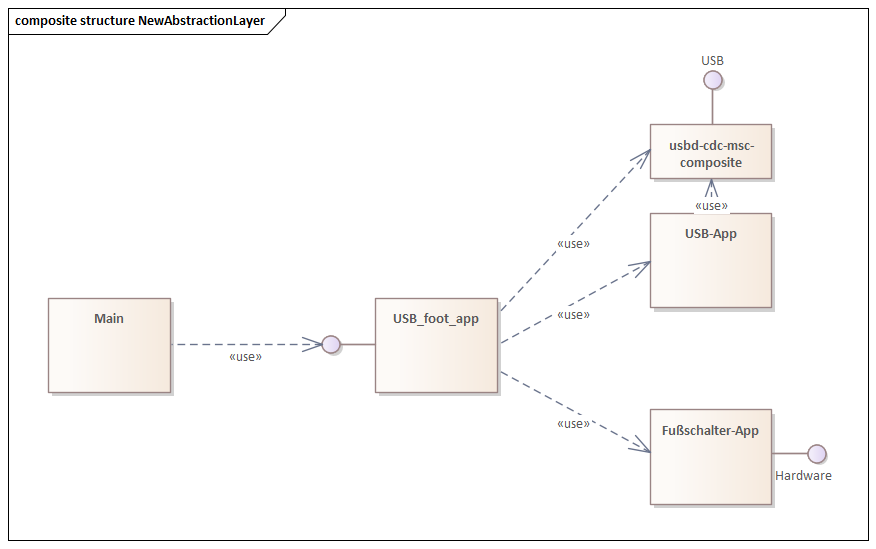
\includegraphics[width=\textwidth]{figures/NewAbstractionLayer.png}
	\caption{Neue Abstraktionsschicht}
\end{figure}

\subsubsection{USB-HID}
Ein Feature, das sowohl für die USB-App als auch für den Fußschalter implementiert werden soll, ist das Human Interface Device (HID). In diesem Modus gibt die Anwendung die Messergebnisse nicht mehr über den virtuellen COM-Port aus, sondern ist über USB als Tastatur mit Computer verbunden und gibt die Zahlen des Ergebnisses als Tastendrücke, gefolgt von einem konfigurierbaren Terminierungszeichen, ein. Dadurch können Messungen einfach in Excel oder einem Texteditor aufgefangen werde. 

In einem ersten Schritt wird grundsätzlich die Funktionalität und das Messergebnis zusätzlich zur Ausgabe über den virtuellen COM-Port ausgegeben. Dies ist eine Vorbereitung für die Implementierung der verschiedenen Operationsmodi. 

\subsubsection{BLE-HID}
Ein weiterer Modus, in dem der Fußschalter arbeiten soll, ist HID über BLE. Das bedeutet, dass sich der Fußschalter als Tastatur im kabellosen Zustand präsentieren kann und wie bei HID über USB die Messergebnisse als Tastatur Tastendrücken in einen Editor oder Excel eintippt. Dazu muss das Gerät nun zusätzlich zur Central Rolle in der Peripheral Rolle agieren. Dazu muss einerseits das Advertising korrekt konfiguriert werden und in den bestehenden Code des Peripheral Verbindungsaufbaus, die Fußschalter Applikation eingebunden werden. Für das eigentliche Schreiben des Messergebnisses über BLE wird gibt es bereits bestehenden Funktionen und diese müssen nur in der Fußschalter Applikation aufgerufen werden. Erste Tests zeigen, dass die Geschwindigkeit der Übertragung, einerseits der Dauer bis angefangen wird das Messergebnis zu schreiben und anderseits wie schnell die einzelnen Tastendrücke erfolgen, stark von USB oder einen mitlaufenden Debugger beeinträchtigt wird. Beides sollte im eigentlichen Anwendungsfall dieses Modus nicht vorhanden sein. 

\subsubsection{BLE-Windows-App}
Der letzte Modus, in dem der Fußschalter agieren soll, ist als ein an die HCT-Windows-App angebundenes Gerät. Dabei soll das Signal der Betätigung des Tasters als eine HCT-Nachricht an die Windows-App gesendet werden, welchen dann ein Messergebnis bei den mit ihr verbundenen Messgeräten triggert. Dazu muss ein HCT-Model für den Fußschalter geschaffen werden. Das Model stellt folgende Werte bereit:
\begin{itemize}
	\item Device Class
	\item Protocol type, version 
	\item Version of Hardware, Software, BLE
	\item Battery level, status
	\item Reset 
\end{itemize}

Werte des Config.ini Konfigurationsfiles:
\begin{itemize}
	\item Operating Mode 
	\item CDC protocol 
	\item HID Keyboard Language ID 
	\item HID data set seperator 
	\item HID number seperator
	\item HID single key 
\end{itemize}

Für die Übertragung des eigentlichen Signals, dass der Fußschalter betätigt wurde, muss eine HCT-Charakteristik angelegt werden, auf welche die HCT-Windows-App sich subscriben kann. Über diese Charakteristik wird sie dann über die Betätigung des Tasters notifiziert. Im Advertising muss sich der Fußschalter dann nicht als Tastatur, sondern als HCT-Fußschalter erkenntlich zeigen. Dazu  


\subsection{Allgemeine Erweiterungen}

\subsubsection{Trennung der Projekte}
Die Grundlage des Projekts nRF52\_base wird unterschiedlichsten Produkte eingesetzt. Im Drehmomentprüfgerät als Central Device und im Drehmomentschlüssel als Peripheral Device für übergeordnete Device Applikationen mit der über serielle UART kommuniziert wird. Im USB-Dongle und im HCT-Fußschalter ist das Basisprojekt direkt auf einem Chip mit der Anwendung des Dongles und des Fußschalters. 

Da im Dongle und im Fußschalter die UART-Kommunikation nicht benötigt wird, während im Drehmomentprüfgerät und im Drehmomentschlüssel die Anwendung des Dongles nicht benötigt wird, werden entsprechende Codestellen durch Compilerschalter aufgetrennt. So wird gewährleistet, dass für alle Projekte nur einen Codebasis mainted werden muss. 

Die USB-App ist bereits gut gekapselt von dem Basisprojekt. Folgende Funktionsaufrufe müssen abgetrennt werden.\\
\\
Main File:
\begin{itemize}
	\item Usb\_app\_init() 
	\item Usb\_app\_process() 
\end{itemize}
Central File:
\begin{itemize}
	\item Alle Aufrufe zu „app\_uart\_put“ 
	\item Alle USB App Callbacks 
\end{itemize}

In einer ersten Ausbaustufe wird mit einem Compilerschalter „UART“ in Central File die Aufrufe zur UART abgetrennt, während mit einem Compilerschalter „USB\_APP“ die Funktionalität der USB-App gekapselt wird. Letztendlich sollte die Verwendung der UART durch geeignete syntaktische Mittel weiter gekapselt werden. 
Nach Trennung der beiden Projekte durch Compilerschalter zeigt sich, dass die compilierten Binärfiles zwar gleich groß sind, jedoch nicht übereinstimmen, was eine weitere Analyse nach sich zieht.

\subsubsection{Verbesserung Verbindungsaufbau}
Im derzeitigen Zustand, sobald die Konfigurationsdatei eingelesen ist, geht die App die zu verbindenden Geräte durch und überprüft jeweils deren Flag über den Verbindungszustand. Wird ein Gerät gefunden, das nicht verbunden ist, wird das Scanning gestartet. Wird ein Gerät von dem Central gefunden, wird der Verbindungsaufbau angestoßen. Sobald die Service discovery stattgefunden hat, wird sich auf die HCT-Charakteristik subscribed und das Connection Handle des Geräts aus dem Central Device übernommen. \\

Eine tiefere Analyse zeigt jedoch, dass zwischen dem Anstoß des Verbindungsaufbau und dem Subscribing auf die HCT-Charakteristik ein weiterer Zustand eingenommen wird. Wenn der Verbindugsaufbau vollzogen wurde, wird ein Flag übermittelt, sowie erstmals dem Gerät das Connection Handle zugeordnet. Ebenfalls kann in diesem Zustand bereits ein Disconnect stattfinden, was im derzeitigen Zustand nicht in der USB-App nachvollzogen werden kann, da das Connection Handle noch nicht gespeichert wurde. Daher muss dieser Zustand programmatisch abgebildet werden.

\begin{figure}[H] 
	\centering
	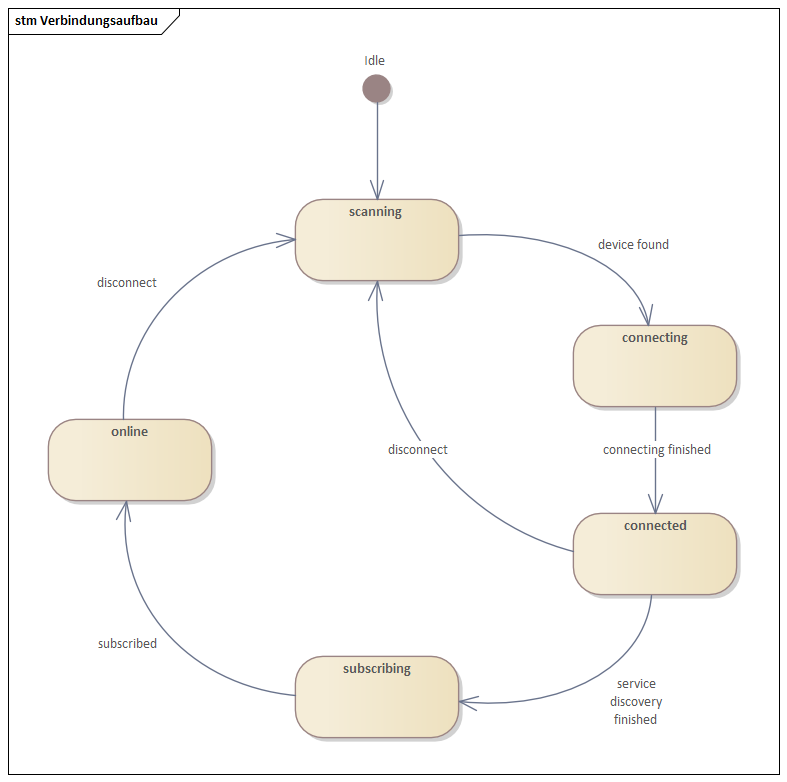
\includegraphics[width=\textwidth]{figures/Verbindungsaufbau.png}
	\caption{Aufbau USB-Dongle App}
\end{figure}

\subsubsection{Optimierung Abfrage Messeinheit} 
Im derzeitigen Stand der USB-Dongle App muss die Anwendung bei Drehmomentschlüsseln und Messuhren der Marke Holex jedes Mal, wenn sie ein Messergebnis erhält, die Einheit der Messung abfragen. 

Bei Drehmomentschlüsseln der Marke Garant wird ein Datenblock mit der Messeinheit kurz nach erhalten des Messergebnisses empfangen. Diese Nachricht bezieht sich jedoch auf die derzeitig eingestellte Messeinheit, welche im Fall eines Arbeitsablaufs mit sich ändernden Einheiten, die Einheit für die nächste Messung ist. In diesem Fall gibt die USB-Dongle App die falsche Einheit über USB-CDC aus. 

In beiden Fällen sendet der Drehmomentschlüssel automatisch bei einer Änderung der Messkonfiguration einen Datenblock mit der Messeinheit an die Dongle App. 

Die Kontrolle der Messeinheit kann daher verbessert werden, indem die derzeitig eingestellte Messeinheit nach dem Verbindungsaufbau einmal abgefragt wird und für jedes verbundene Gerät gespeichert wird. Bei einer Änderung der Messeinheit wird die Dongle App notifiziert und die gespeicherte Einheit aktualisiert. Dadurch wird eine fehlerhafte Einheit in der Ausgabe über USB-CDC vermieden und die Anzahl an Nachrichten der Dongle-App an das Messgerät verringert.

\begin{figure}[H] 
	\centering
	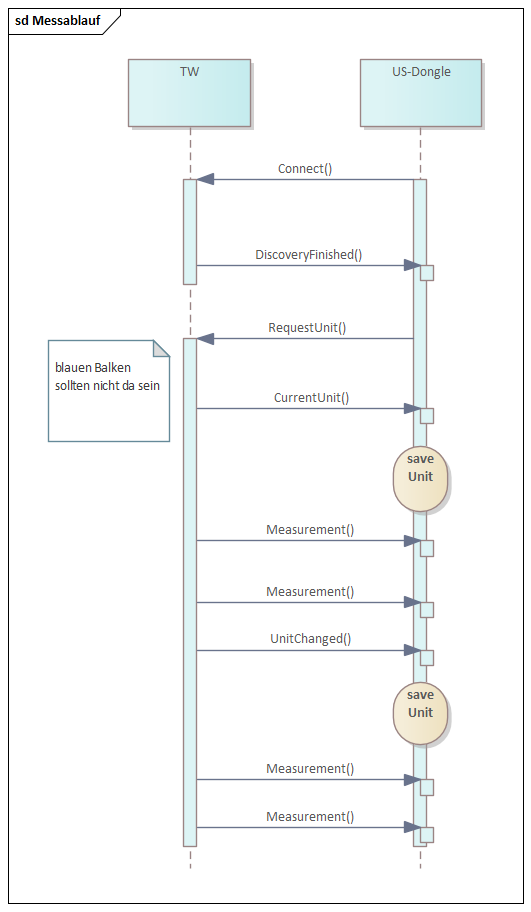
\includegraphics[width=\textwidth]{figures/Messablauf.png}
	\caption{Messablauf}
\end{figure}

